\documentclass{article}
\usepackage[margin=1in]{geometry}
\usepackage[linesnumbered,ruled,vlined]{algorithm2e}
\usepackage{amsfonts}
\usepackage{amsmath}
\usepackage{amssymb}
\usepackage{amsthm}
\usepackage{enumitem}
\usepackage{fancyhdr}
\usepackage{hyperref}
\usepackage{minted}
\usepackage{multicol}
\usepackage{pdfpages}
\usepackage{standalone}
\usepackage[many]{tcolorbox}
\usepackage{tikz-cd}
\usepackage{transparent}
\usepackage{xcolor}
% \tcbuselibrary{minted}

\author{Nathan Solomon}

\newcommand{\fig}[1]{
    \begin{center}
        \includegraphics[width=\textwidth]{#1}
    \end{center}
}

% Math commands
\renewcommand{\d}{\mathrm{d}}
\DeclareMathOperator{\id}{id}
\DeclareMathOperator{\im}{im}
\DeclareMathOperator{\proj}{proj}
\DeclareMathOperator{\Span}{span}
\DeclareMathOperator{\Tr}{Tr}
\DeclareMathOperator{\tr}{tr}
\DeclareMathOperator{\ad}{ad}
\DeclareMathOperator{\ord}{ord}
%%%%%%%%%%%%%%% \DeclareMathOperator{\sgn}{sgn}
\DeclareMathOperator{\Aut}{Aut}
\DeclareMathOperator{\Inn}{Inn}
\DeclareMathOperator{\Out}{Out}
\DeclareMathOperator{\stab}{stab}

\newcommand{\N}{\ensuremath{\mathbb{N}}}
\newcommand{\Z}{\ensuremath{\mathbb{Z}}}
\newcommand{\Q}{\ensuremath{\mathbb{Q}}}
\newcommand{\R}{\ensuremath{\mathbb{R}}}
\newcommand{\C}{\ensuremath{\mathbb{C}}}
\renewcommand{\H}{\ensuremath{\mathbb{H}}}
\newcommand{\F}{\ensuremath{\mathbb{F}}}

\newcommand{\E}{\ensuremath{\mathbb{E}}}
\renewcommand{\P}{\ensuremath{\mathbb{P}}}

\newcommand{\es}{\ensuremath{\varnothing}}
\newcommand{\inv}{\ensuremath{^{-1}}}
\newcommand{\eps}{\ensuremath{\varepsilon}}
\newcommand{\del}{\ensuremath{\partial}}
\renewcommand{\a}{\ensuremath{\alpha}}

\newcommand{\abs}[1]{\ensuremath{\left\lvert #1 \right\rvert}}
\newcommand{\norm}[1]{\ensuremath{\left\lVert #1\right\rVert}}
\newcommand{\mean}[1]{\ensuremath{\left\langle #1 \right\rangle}}
\newcommand{\floor}[1]{\ensuremath{\left\lfloor #1 \right\rfloor}}
\newcommand{\ceil}[1]{\ensuremath{\left\lceil #1 \right\rceil}}
\newcommand{\bra}[1]{\ensuremath{\left\langle #1 \right\rvert}}
\newcommand{\ket}[1]{\ensuremath{\left\lvert #1 \right\rangle}}
\newcommand{\braket}[2]{\ensuremath{\left.\left\langle #1\right\vert #2 \right\rangle}}

\newcommand{\catname}[1]{{\normalfont\textbf{#1}}}

\newcommand{\up}{\ensuremath{\uparrow}}
\newcommand{\down}{\ensuremath{\downarrow}}

% Custom environments
\newtheorem{thm}{Theorem}[section]

\definecolor{probBackgroundColor}{RGB}{250,240,240}
\definecolor{probAccentColor}{RGB}{140,40,0}
\newenvironment{prob}{
    \stepcounter{thm}
    \begin{tcolorbox}[
        boxrule=1pt,
        sharp corners,
        colback=probBackgroundColor,
        colframe=probAccentColor,
        borderline west={4pt}{0pt}{probAccentColor},
        breakable
    ]
    \color{probAccentColor}\textbf{Problem \thethm.} \color{black}
} {
    \end{tcolorbox}
}

\definecolor{exampleBackgroundColor}{RGB}{212,232,246}
\newenvironment{example}{
    \stepcounter{thm}
    \begin{tcolorbox}[
      boxrule=1pt,
      sharp corners,
      colback=exampleBackgroundColor,
      breakable
    ]
    \textbf{Example \thethm.}
} {
    \end{tcolorbox}
}

\definecolor{propBackgroundColor}{RGB}{255,245,220}
\definecolor{propAccentColor}{RGB}{150,100,0}
\newenvironment{prop}{
    \stepcounter{thm}
    \begin{tcolorbox}[
        boxrule=1pt,
        sharp corners,
        colback=propBackgroundColor,
        colframe=propAccentColor,
        breakable
    ]
    \color{propAccentColor}\textbf{Proposition \thethm. }\color{black}
} {
    \end{tcolorbox}
}

\definecolor{thmBackgroundColor}{RGB}{235,225,245}
\definecolor{thmAccentColor}{RGB}{50,0,100}
\renewenvironment{thm}{
    \stepcounter{thm}
    \begin{tcolorbox}[
        boxrule=1pt,
        sharp corners,
        colback=thmBackgroundColor,
        colframe=thmAccentColor,
        breakable
    ]
    \color{thmAccentColor}\textbf{Theorem \thethm. }\color{black}
} {
    \end{tcolorbox}
}

\definecolor{corBackgroundColor}{RGB}{240,250,250}
\definecolor{corAccentColor}{RGB}{50,100,100}
\newenvironment{cor}{
    \stepcounter{thm}
    \begin{tcolorbox}[
        enhanced,
        boxrule=0pt,
        frame hidden,
        sharp corners,
        colback=corBackgroundColor,
        borderline west={4pt}{0pt}{corAccentColor},
        breakable
    ]
    \color{corAccentColor}\textbf{Corollary \thethm. }\color{black}
} {
    \end{tcolorbox}
}

\definecolor{lemBackgroundColor}{RGB}{255,245,235}
\definecolor{lemAccentColor}{RGB}{250,125,0}
\newenvironment{lem}{
    \stepcounter{thm}
    \begin{tcolorbox}[
        enhanced,
        boxrule=0pt,
        frame hidden,
        sharp corners,
        colback=lemBackgroundColor,
        borderline west={4pt}{0pt}{lemAccentColor},
        breakable
    ]
    \color{lemAccentColor}\textbf{Lemma \thethm. }\color{black}
} {
    \end{tcolorbox}
}

\definecolor{proofBackgroundColor}{RGB}{255,255,255}
\definecolor{proofAccentColor}{RGB}{80,80,80}
\renewenvironment{proof}{
    \begin{tcolorbox}[
        enhanced,
        boxrule=1pt,
        sharp corners,
        colback=proofBackgroundColor,
        colframe=proofAccentColor,
        borderline west={4pt}{0pt}{proofAccentColor},
        breakable
    ]
    \color{proofAccentColor}\emph{\textbf{Proof. }}\color{black}
} {
    \qed \end{tcolorbox}
}

\definecolor{noteBackgroundColor}{RGB}{240,250,240}
\definecolor{noteAccentColor}{RGB}{30,130,30}
\newenvironment{note}{
    \begin{tcolorbox}[
        enhanced,
        boxrule=0pt,
        frame hidden,
        sharp corners,
        colback=noteBackgroundColor,
        borderline west={4pt}{0pt}{noteAccentColor},
        breakable
    ]
    \color{noteAccentColor}\textbf{Note. }\color{black}
} {
    \end{tcolorbox}
}


\fancyhf{}
\setlength{\headheight}{24pt}

\date{\today}
\title{Physics 105B Lecture Notes, Fall 2024}

\begin{document}
\maketitle

The class textbook is \textit{Classical Mechanics of Particles and Systems, 5th edition} by Marion \& Thornton. These notes are a supplement for the textbook, not a replacement, so I won't cover everything from the course.

\tableofcontents
\section{Review of Lagrangian mechanics (physics 105A)}
\subsection{Calculus of variations}
Use catenary and brachiostrome as examples
\subsection{Least action principle}
\subsection{Generalized momenta}
\subsection{Lagrange multipliers, forces from constraints}

\section{Phase diagrams}
For lots of systems, the state can be described by generalized positions ($q_1, q_2, \dots$) and generalized velocities ($\dot{q_1}, \dot{q_2}, \dots$). For example, the state of a pendulum at any time can be described by the vector
\[ \begin{bmatrix}
    \theta \\
    \dot{\theta}
\end{bmatrix}, \]
and if we know the state, we can calculate the rate of change of the state. That is,
\[ \begin{bmatrix}
    \dot{\theta} \\
    \ddot{\theta}
\end{bmatrix} \]
is a function of the state. We can visualize this as a vector field, where $x = \theta$ and $y = \dot{\theta}$. One amazing tool for animating vector fields is
\url{https://anvaka.github.io/fieldplay/}
\par
For the pendulum example, copy this code:
\begin{lstlisting}[language=C,frame=single]
// p.x and p.y are current coordinates
// v.x and v.y is a velocity at point p
vec2 get_velocity(vec2 p) {
  vec2 v = vec2(0., 0.);
  v.x = p.y;
  v.y = cos(p.x);
  return v;
}
\end{lstlisting}
\fig{pendulum.png}

For a Van der Pol oscillator, copy in this code, and experiment with changing $\mu$ (mu):
\begin{lstlisting}[language=C,frame=single]
float mu = 1.;
vec2 get_velocity(vec2 p) {
  return vec2(p.y, mu*(1.-p.x*p.x)*p.y-p.x);
}
\end{lstlisting}
Here is a Van der Pol oscillator with $\mu = 1$:
\fig{VanDerPol.png}

\section{Rotating reference frames}
Chapter 10 in the textbook. Copy example 10.5 (Foucault pendulum) to these notes

\section{Moment of inertia tensor}
Compare the off-diagonal elements (``products of inertia") to the formula for Pearson's correlation coefficient, which measures how much stuff is on a diagonal line between the $x$ and $y$ axes. Use this to give an intuitive explanation of what diagonalizing $I$ represents.
\subsection{Stress tensor}
A lot of your intuition for the moment of inertial tensor can be applied to the stress tensor $\sigma$, which is another contravariant, symmetric, second-order tensor. It represents the forces on each point in a material. Thinking of it as a 3 by 3 matrix, the diagonal elements represent the tensile stress along each axis. So for example, $\sigma_{1,1}$ would be positive if the material it being stretched along the $x$ axis at that point, and negative if it is being squished along the $x$ axis at that point.
\par
The off-diagonal elements of $\sigma$ represent shear forces. For example, if $\sigma_{1,2} = \sigma_{2,1} > 0$, then there is some shearing force in the $x,y$ plane. Such a force could also be treated as a pulling force in the direction of the unit vector $\pm \frac{1}{\sqrt{2}} (\hat{x} + \hat{y})$. By treating all of the shearing forces as pulling or squishing along some axis other than $\hat{x}$, $\hat{y}$, or $\hat{z}$, we can describe the stress tensor with just the tensile stress along those 3 axes, which we can ensure are orthogonal, because $\sigma$ is symmetric. This is equivalent to diagonalizing the stress tensor.
\par
To intuitively understand these off-diagonal elements, imagine a square pice of sheet metal lying in the $x,y$ plane, with one edge flushed to the $x$ axis and another flushed to the $y$ axis. Then apply a shear force $F \propto y \hat{x}$ to it, which points along the $x$ axis and is proportional to the $y$ coordinate. This force acts to stretch the square into a rhombus, effectively pulling (that is, applying tensile stress) in the $\frac{1}{\sqrt{2}} (\hat{x} + \hat{y})$ direction.
\par
Stress has units of force per area. One Pascal is a Newton per meter squared, and one atmosphere is about $101.3$ kilopascals. If the stress tensor is some scalar $\sigma_{1,1}$ times the identity tensor, then we can say that the pressure is $-\sigma_{1,1}$. Air pressure at sea level is very close to 1 atm, and air pressure pretty much decays exponentially with altitude.
\begin{center}
    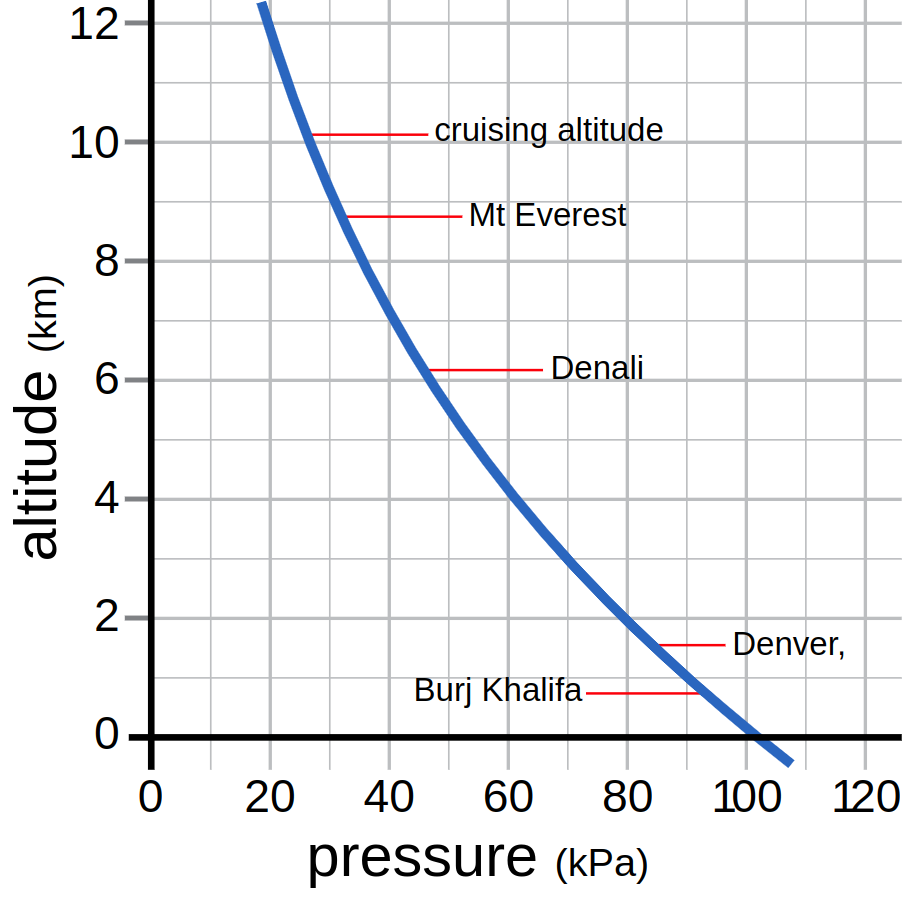
\includegraphics[width=0.5\textwidth]{pressure.png}
\end{center}

\section{Euler angles}

\section{Synchronized/Coupled oscillators (chapter 12)}
Include links to and screenshots of synchronizing oscillators from the ``Explorable explanations" website (although that's different from the oscillators we are talking about here).

\end{document}
